\chapter{Classification}

In this task, our goal was to create a classifier which, given an incident, would predict the presence of a fatality. 

Two different classifiers have been tested: a Decision Tree, for it's interpretable nature, and a Neural Network, for it's ability to capture complex relationships between the features.

\section{Methods}

Since the target variable comes from the dataset in the form of \highlighttext{n\_killed} which is the number of fatalities, it was necessary to transform it into a binary variable (\highlighttext{isKilled}) and to drop the original one and all the features directly derivating from it.

\subsection{Feature Selection}

Some early tests showed nearly perferct results from the classifiers. Analyzing the Decision Tree it was easy to see that the classifier was obtaining the value of \highlighttext{n\_killed} from \highlighttext{n\_participants - n\_injured - n\_unharmed - n\_arrested}.

To avoid this problem, \highlighttext{n\_participants} and all the features that would allow to obtain it were dropped.

Later tests showed that the classifier was still \textit{cheating} when \highlighttext{n\_injured} == \highlighttext{n\_unharmed} == \highlighttext{n\_arrested} == 0; in this case, given that \highlighttext{n\_participants} $\geq 1$, the value of \highlighttext{n\_killed} would be $\geq 1$. To avoid artificially inflating the scores, the datapoints where this condition was met were dropped. 

\subsection{Scaling}

For the Decision Tree classifier, no scaling was necessary, so it was not performed to keep the interpretability of the model.

For the Neural Network, the dataset was scaled using the \highlighttext{StandardScaler} from SKLearn.

\subsection{Training-Validation-Test split}

The dataset was split into three parts: training ($70\%$), validation ($15\%$) and test ($15\%$). The training set was used to train the classifier, the validation set was used evaluate the difference in performance between different classifiers and to tune the hyperparameters, and the test set was used to evaluate the final performance of the classifiers.

\subsection{Balancing}

The dataset is unbalanced, with around $75\%$ of incidents having no fatalities. This could lead to a classifier that always predicts no fatalities. To avoid this problem the dataset was balanced using the \highlighttext{SMOTE}\cite{chawla2002smote} algorithm on the training set, and with upsampling with replacement on the validation and test sets (to avoid testing on syntetic data).


\section{Decision Tree}

SKLearn's Decision Tree classifier was used. To try to avoid overfitting, a Grid Search was performed.

Despite this, the best classifier obtained had an F1 score of $0.93$ on the training set, while on the validation set it had an F1 score of $0.72$.

\begin{figure}[h]
    \centering
    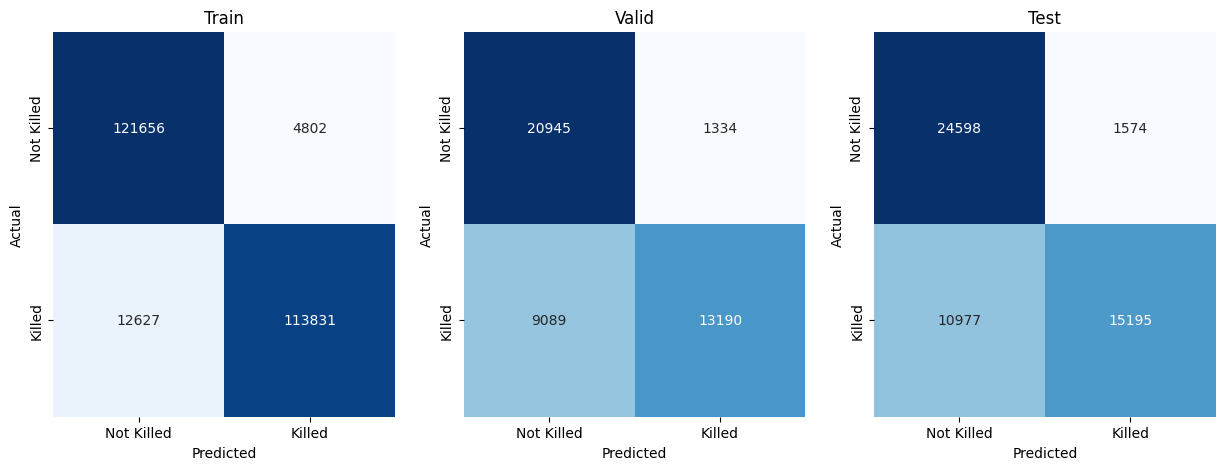
\includegraphics[width=\textwidth]{images/Clustering/decision_tree_cm.png}
    \caption{Decision Tree confusion matrix of the training, validation and test sets.}
    \label{fig:decision_tree_cm}
\end{figure}

On Figure \ref{fig:decision_tree_cm} the confusion matices of the training, validation and test sets can be analyzed. While still having positive results, the classifier is clearly overfitting.

The final test F1 score was $0.71$. Figure \ref{fig:decision_tree} shows the first three levels of the Decision Tree.

\begin{figure}[h]
    \centering
    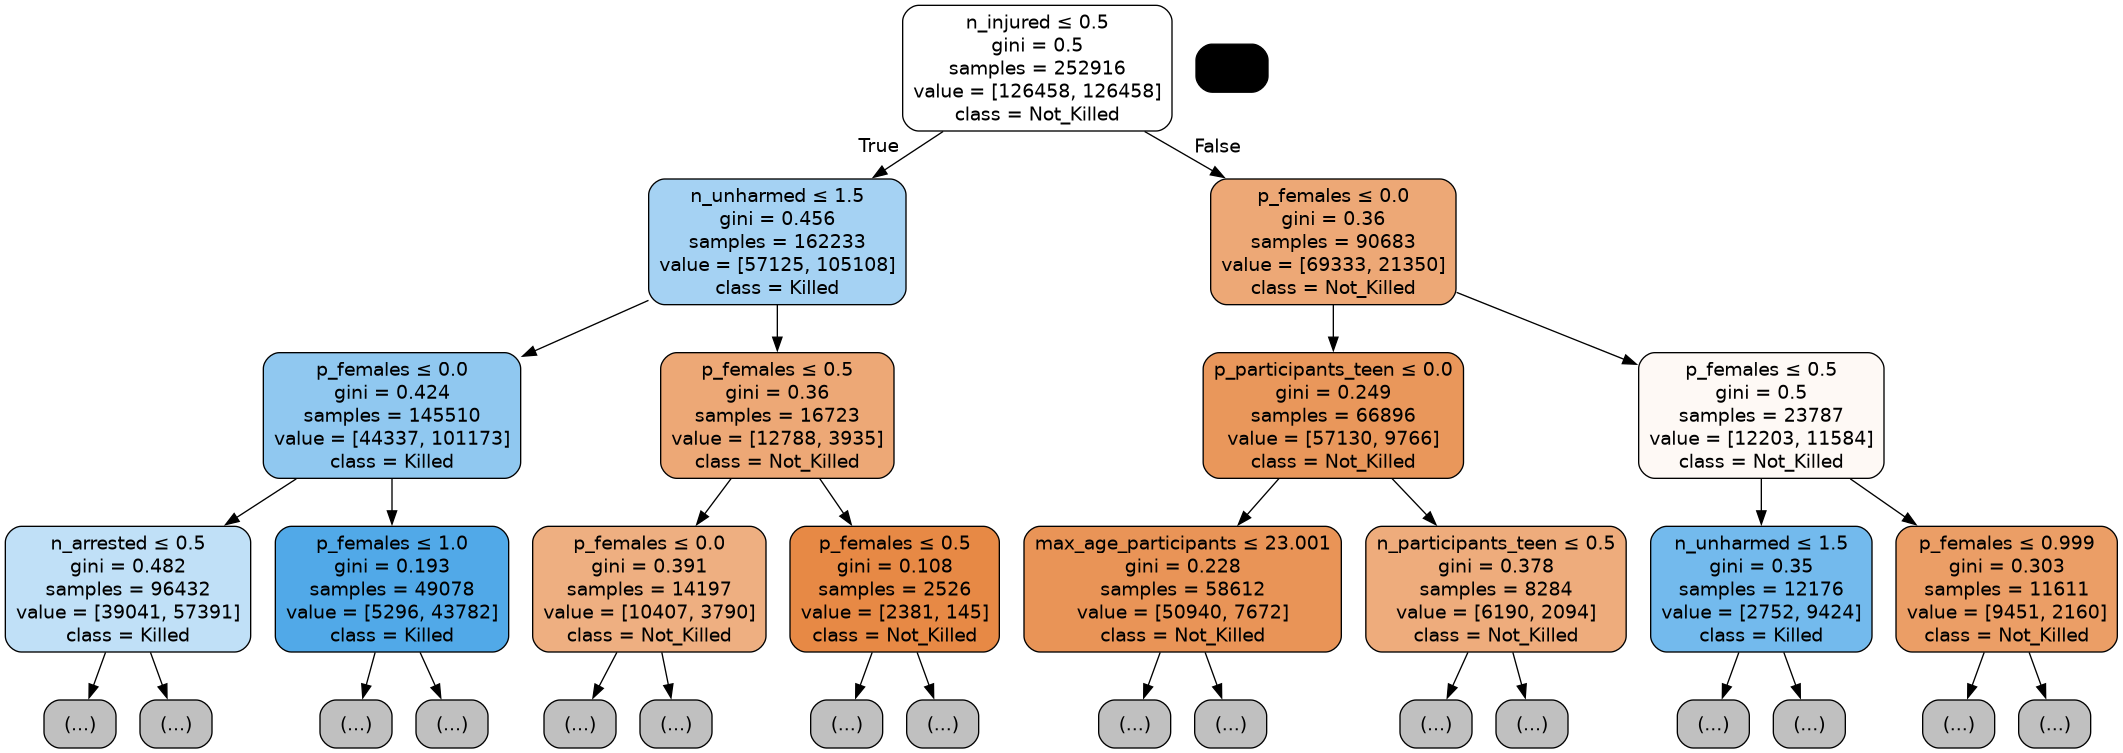
\includegraphics[width=\textwidth]{images/Clustering/decision_tree.png}
    \caption{Decision Tree.}
    \label{fig:decision_tree}
\end{figure}

\section{Neural Network}

A Neural Network was trained hoping that it would find hidden relations in the data. The architecture used was the following:

\begin{itemize}
    \item Input layer with 23 neurons (one for each feature)
    \item 4 Hidden layers with [32, 16, 8, 4] neurons and Sigmoid activation function, followed by a 10\% dropout rate
    \item Output layer with 2 neurons and Softmax activation function
\end{itemize}

The model was trained with an Early Stopping callback, which stopped the training if the validation score did not improve for 10 validation steps.

The Early Stopping kicked in at the 13000th epoch, with a training F1 score of $0.82$ and a validation F1 score of $0.78$.

\begin{figure}[h]
    \centering
    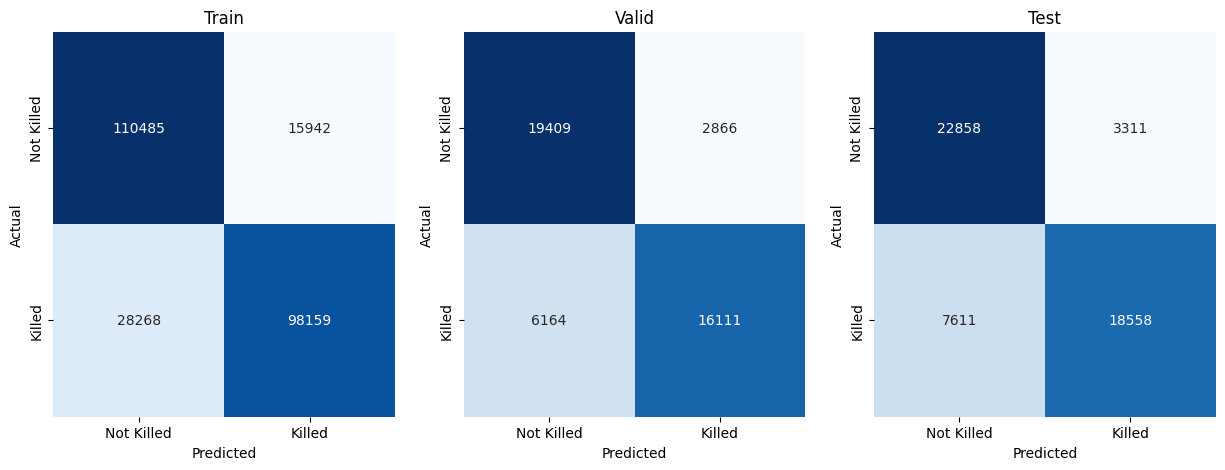
\includegraphics[width=\textwidth]{images/Clustering/nn_cm.png}
    \caption{Neural Network confusion matrix of the training, validation and test sets.}
    \label{fig:nn_cm}
\end{figure}

Figure \ref{fig:nn_cm} shows the confusion matrices of the training, validation and test sets. The final test F1 score was $0.77$. 

\section{Comparison}

\begin{figure}[h]
    \centering
    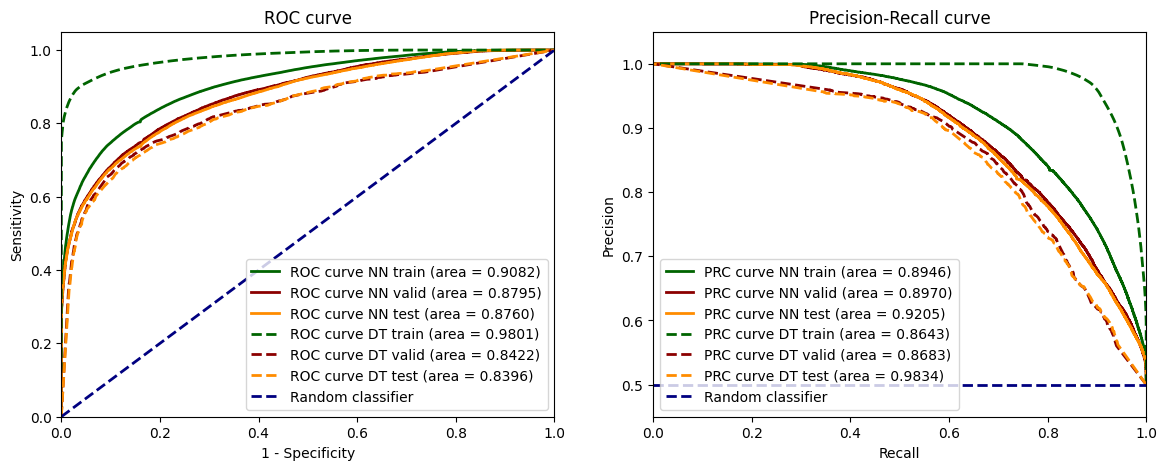
\includegraphics[width=\textwidth]{images/Clustering/roc-prc.png}
    \caption{ROC and Precision-Recall curves of the Decision Tree and Neural Network compared.}
    \label{fig:roc}
\end{figure}

Figure \ref{fig:roc} shows the ROC and Precision-Recall curves of the Decision Tree and Neural Network compared. 

The Neural Network has a slight advantage over the Decision Tree, with higher scores on the test set, but not significat enough to mark it as better suited for the task.

\begin{quotation}
    \small
    It is important to note that due to hardware limitations, the search for the best hyperparameters was not exhaustive, and it is possible that better results could be obtained with a more thorough search.
\end{quotation}